\section{Systemtechnik}
\subsection{Modellbildung}
	Hinweise zum aufstellen der Differentialgleichung eines Systems:
	\begin{mdframed}[style=exercise]
		\begin{enumerate}
			\item Bestimmung der Ein- und Ausgangsgrößen
			\item Suche nach dem beschreibenden Gleichgewicht
			\item In der Gleichung dürfen nur Konstanten, sowie die Ein- und
				Ausgangsgrößen in beliebiger Ableitung vorkommen
			\item Andere Variablen müssen durch erlaubte Größen ersetzt werden\\
				\footnotesize
				(Dazu können i.a. physikalische Gleichungen benutzt werden)
		\end{enumerate}
	\end{mdframed}

\subsection{Signalflussplan/Blockschaltbild}
	Erzeugung des Signalflussplans aus der Zugehörigen DGL.
	\begin{mdframed}[style=exercise]
		\begin{enumerate}
			\item für technische Realisierung gilt: \(m \le n\);

			\item DGL. nach höchster Ableitung der Ausgangsgröße auflösen

			\item höchste Ableitung der Ausgangsgröße geht auf den Eingang des ersten Integrators\\
				\footnotesize
				(Laplace-Trans ersetzt Integrieren mit \(\frac{1}{s}\))
		\end{enumerate}
	\end{mdframed}
	\begin{center}
		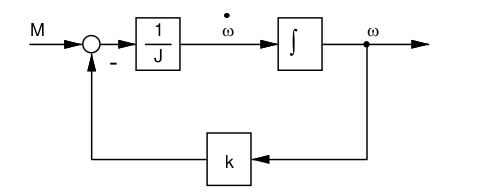
\includegraphics[width=0.96\columnwidth]{Figures/systemtechnik/Signalflussplan12.png}
	\end{center}

	\begin{mdframed}[style=exercise]
		Erzeugung des Signalflussplans eines Systems mit der DGL.:
		\begin{align*}
			& a_{n} \overset{(n)}{x}_{a}+\ldots+a_{2} \ddot{x}_{a}+a_{1} \dot{x}_{a}+a_{0} x_{a} \\
			= & b_{m} \overset{(m)}{x}_{e}+\ldots+b_{2} \ddot{x}_{e}+b_{1} \dot{x}_{e}+b_{0} x_{e}
		\end{align*}
		\centering
		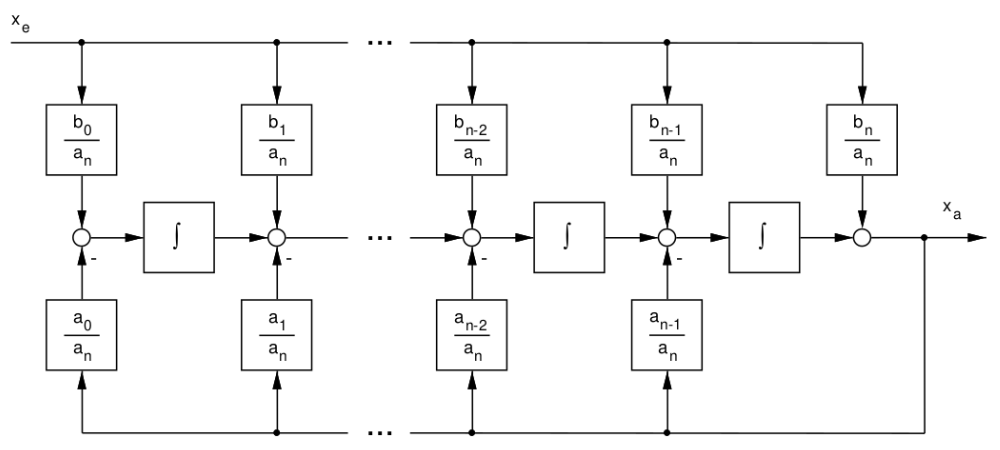
\includegraphics[width=\columnwidth]{Figures/systemtechnik/SFmitDGL.png}
		Falls \(m < n \), sind alle höheren \(b_\mu = 0\) zu wählen.
	\end{mdframed}

\subsection{Übertragungsfunktion F(s)}
	\begin{align*}
		F(s) = \frac{X_a(s)}{X_e(s)}
	\end{align*}

\subsubsection{F(s) aus DGL}
	
\begin{mdframed}[style=exercise]
	\begin{align*}
		& a_{n} \overset{(n)}{x}_{a}+\ldots+a_{1} \dot{x}_{a}+a_{0} x_{a} = b_{m} \overset{(m)}{x}_{e}+\ldots+b_{1} \dot{x}_{e}+b_{0} x_{e}\\
		& \Rightarrow F(s) = \frac{b_{m} s^{m}+\ldots+b_{2} s^{2}+b_{1} s+b_{0}}{a_{n} s^{n}+\ldots+a_{2} s^{2}+a_{1} s+a_{0}}
	\end{align*}
\end{mdframed}

\subsubsection{F(s) in Pol- und Nullstellenform}

\[
	F(s)=Q \cdot \frac{\prod_{\mu=1}^{m}\left(s-s_{N \mu}\right)}{\prod_{v=1}^{n}\left(s-s_{P V}\right)}
	\qquad \texttt{mit } Q = \frac{b_m}{a_n}
\]

\begin{mdframed}[style=exercise]
	Pole in der rechten Halbebene führen zu einem instabilen System. Diese können nicht durch Nullstellen kompensiert werden.

	Pole bewirken ein zeitverzögertes Verhalten. Je weiter links sie sich befinden,
	desto schneller ist der Einschwingvorgang.\\
	$\Rightarrow$ Wenn Pole deutlich weiter links liegen als andere andere, kann man sie ohne
	großen Fehler vernachlässigen.
\end{mdframed}
\begin{mdframed}[style=exercise]
	Nullstellen bewirken ein differenzierendes Verhalten (Beschleunigung des Systems)
	Einfluss weit links in der s-Ebene kann häufig vernachlässigt werden.
\end{mdframed}

\newcolumn
\subsection{Signalflussplan Algebra}
\begin{itemize}[leftmargin=*]
	\item Kettenstruktur:
	      \begin{center}
		      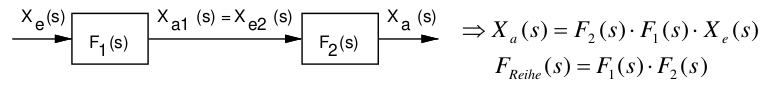
\includegraphics[width=0.9\columnwidth]{Figures/systemtechnik/Kettenstruktur.png}
	      \end{center}

	\item Parallelstruktur:
	      \begin{center}
		      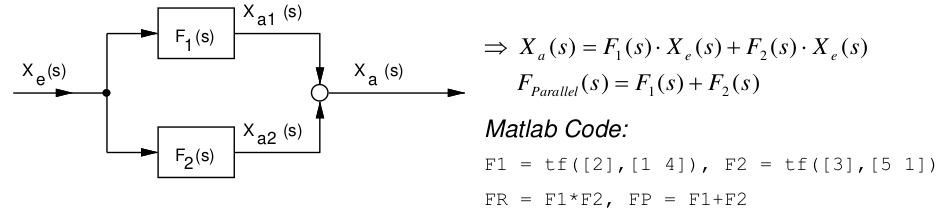
\includegraphics[width=0.9\columnwidth]{Figures/systemtechnik/Parallelstruktur.png}
	      \end{center}

	\item Kreisstruktur:
	      \begin{center}
		      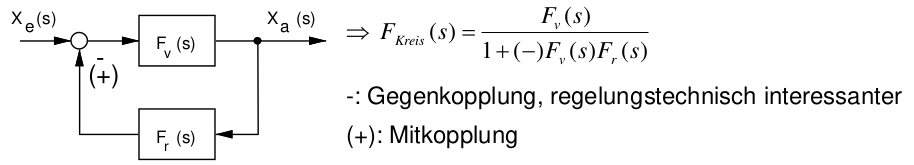
\includegraphics[width=0.9\columnwidth]{Figures/systemtechnik/Kreisstruktur.png}
	      \end{center}

	\item Verschieben einer Additionsstelle:
	      \begin{center}
		      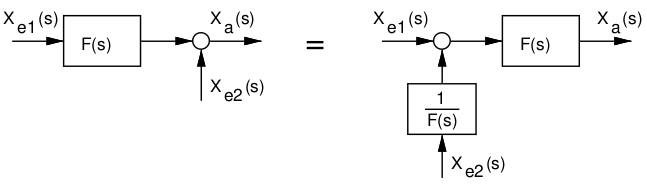
\includegraphics[width=0.9\columnwidth]{Figures/systemtechnik/Verschiebung_Additionsstelle.png}
	      \end{center}

	\item Verschieben einer Verzweigung:
	      \begin{center}
		      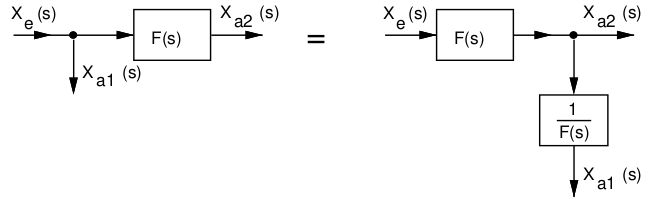
\includegraphics[width=0.9\columnwidth]{Figures/systemtechnik/Verschiebung_Verzweigung.png}
	      \end{center}
\end{itemize}
